\documentclass{article}

\usepackage{phdstyle}
\newcommand{\emi}{\varepsilon}

\begin{document}
Equilibrium level momentum shift is
\[
\Delta\delta_{eq} = \kappa_0\cdot\bkt*{\kappa_1\cdot\frac{\delta_m^2}{2} + \bkt{\frac{\Delta L}{L}}_\beta}.
\]

Betatron motion orbit lengthening is defined by:
\[
\bkt{\frac{\Delta L}{L}}_\beta = \frac{\pi}{2L}\bkt*{\emi_xQ_x + \emi_yQ_y}.
\]

Take two particles (0 \& 1) doing the exact same betatron motion, only one does it in the horizontal plane, the other vertical:
\]
\emi_x^0 = \emi_y^1,~ Q_x^0 = Q_y^1, \emi_y^0 = \emi_x^1 = Q_y^0 = Q_x^1 = 0.
\]

Both have zero momentum offset from the reference particle:
\[
\delta_m^0 = \delta_m^1 = 0.
\]

Their equilibrium level momentum shifts, and hence effective Lorentz factors, are equal
\[
\gamma_{eff} \equiv \gamma_s +\beta_s^2\gamma_s\cdot\Delta\delta_{eq}.
\]

However, their spin precession frequencies, computed as
\[
\vec\W = 2\pi f_{rev} \nu_s \vec n,
\]
are different. (See figures.)

%% \begin{figure}[!h]
%%   \centering
%%   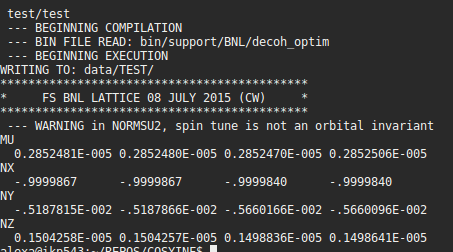
\includegraphics[width=\linewidth]{img/effective_gamma_question_test}
%%   \caption{Left to right particles: -1, +1 mm offset in the x,y coordinate. BNL lattice at FS energy (270.0092 MeV) with a single $10^{-4}$ radians spin kick about the radial axis.}
%% \end{figure}
%% \begin{figure}[!h]
%%   \centering
%%   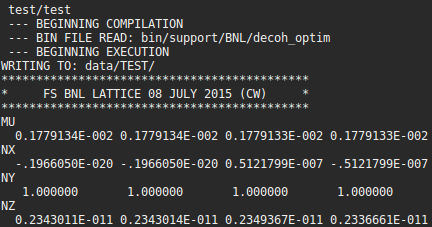
\includegraphics[width=\linewidth]{img/effective_gamma_question_test_non_FS}
%%   \caption{Left to right particles: -1, +1 mm offset in the x,y coordinate. BNL lattice at 274 MeV, no radial spin kicks.}
%% \end{figure}
%% \begin{figure}[!h]
%%   \centering
%%   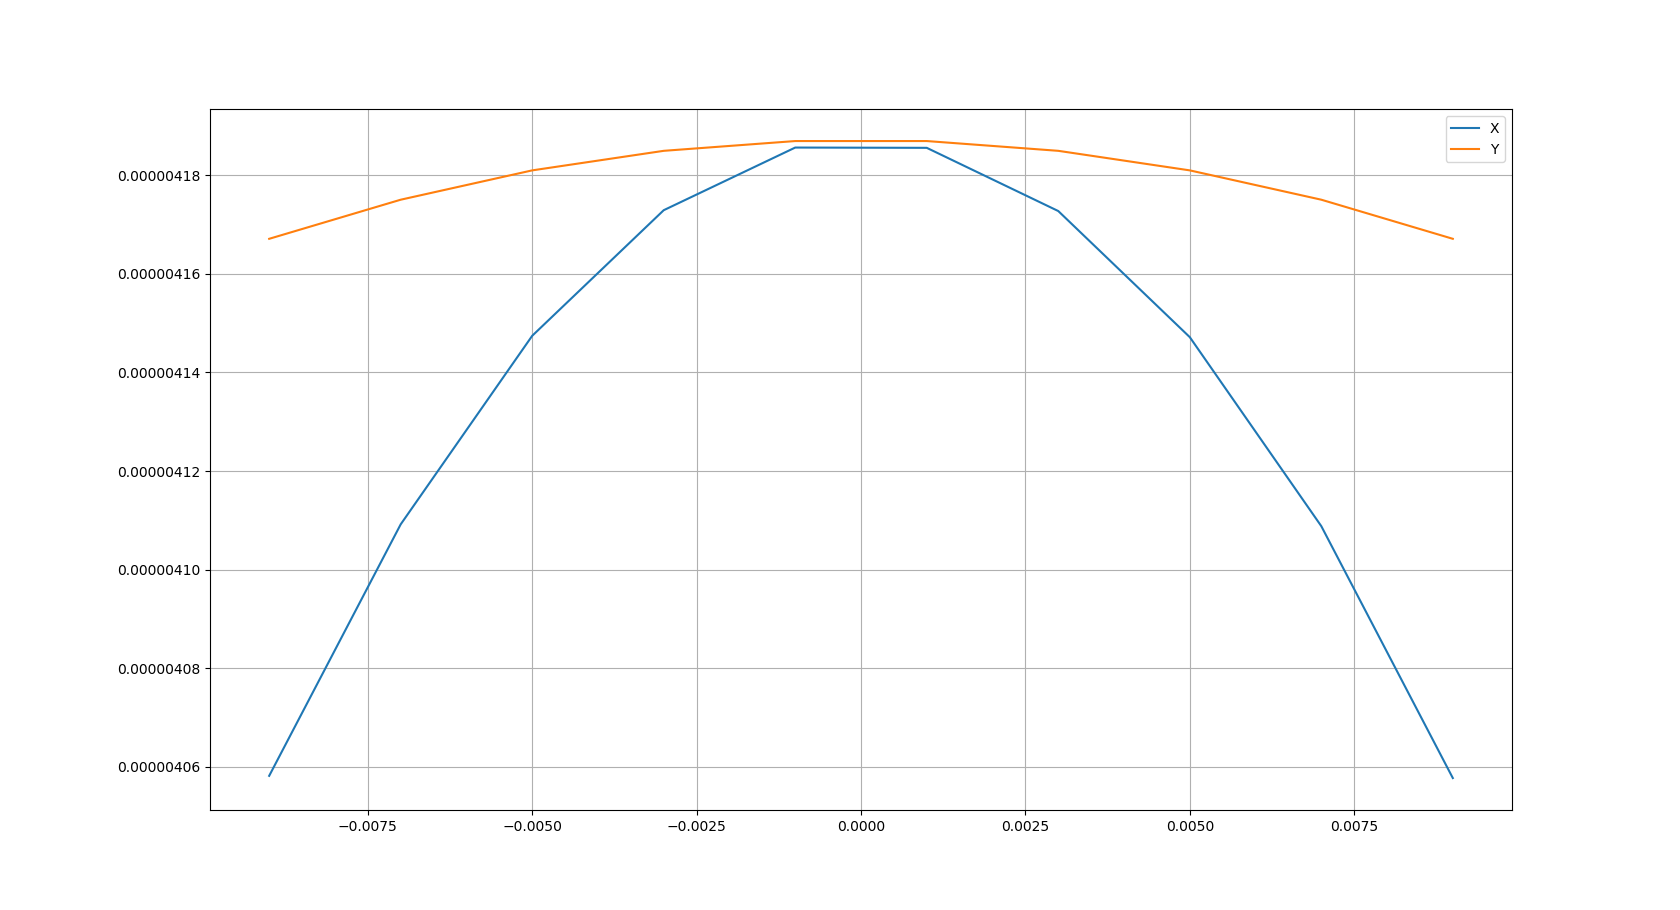
\includegraphics[width=\linewidth]{img/effective_gamma_question_comparison}
%%   \caption{X and Y bunches unoptimized untilted BNL lattice spin tunes (n bar looks stragiht up for all points).}
%% \end{figure}

This is because for the particle oscillating in the horizontal plane, the focusing quadrupole magnetic fields point in the same direction as the guide field, and therefore the kicks done to its spin vector commute with the guide field spin kicks. For the vertically-oscillating particle the commutativity breaks.

Therefore, the statement
\begin{quote}
  Two particles having equal effective Lorentz factors have exactly the same spin precession frequency, regardless of their orbital motion difference.
\end{quote}
is false.

\section{Simulation}
The condition put on the betatron oscillating particles is
\[
\emi_x^0Q_x^0 = \emi_y^1Q_y^1.
\]
The amplitudes of betatron oscillations are
\begin{align*}
  A_x &= \sqrt{\emi_x\beta_x}, \\
  A_y &= \sqrt{\emi_y\beta_y}.
\end{align*}

From the condition, we have:
\[
\emi_y^1 = \emi_x^0\frac{Q_x^0}{Q_y^1},
\]
and hence
\[
A_y = A_x\sqrt{\frac{Q_x}{Q_y}\cdot \frac{\beta_y}{\beta_x}}.
\]

Therefore I inject four particles at 275 MeV, with offsets:
\begin{align*}
  x(0)^{0,1} &= \pm1mm,~ y(0)^{0,1} = 0mm, \\
  x(0)^{2,3} &= 0mm,~ y(0)^{2,3} = \pm1mm \cdot \sqrt{\frac{Q_x^{co}}{Q_y^{co}}\cdot \frac{\beta_y^{co}}{\beta_x^{co}}},
\end{align*}
where $\beta_x^{co},~\beta_y^{co},~Q_x^{co},~Q_y^{co}$ are the beta functions and betatron tunes on the closed orbit (zero-order taylor expansion coefficients).

\begin{figure}[!h]
  \centering
  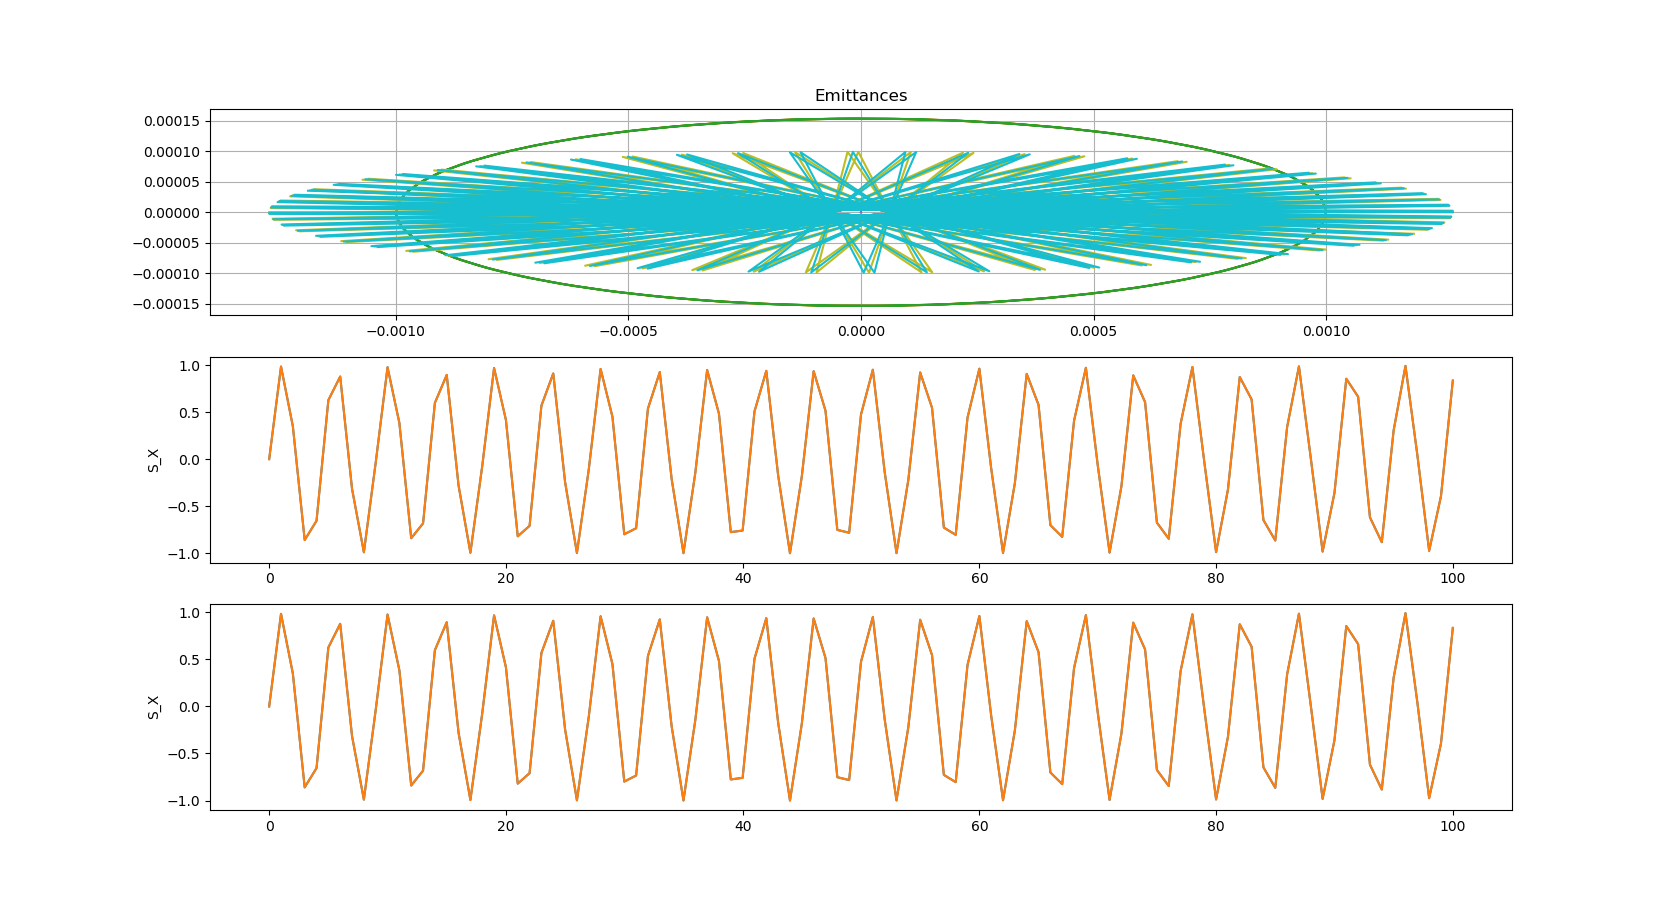
\includegraphics[width=\linewidth]{img/effective_gamma_question_three}
  \caption{}
\end{figure}
\begin{figure}[!h]
  \centering
  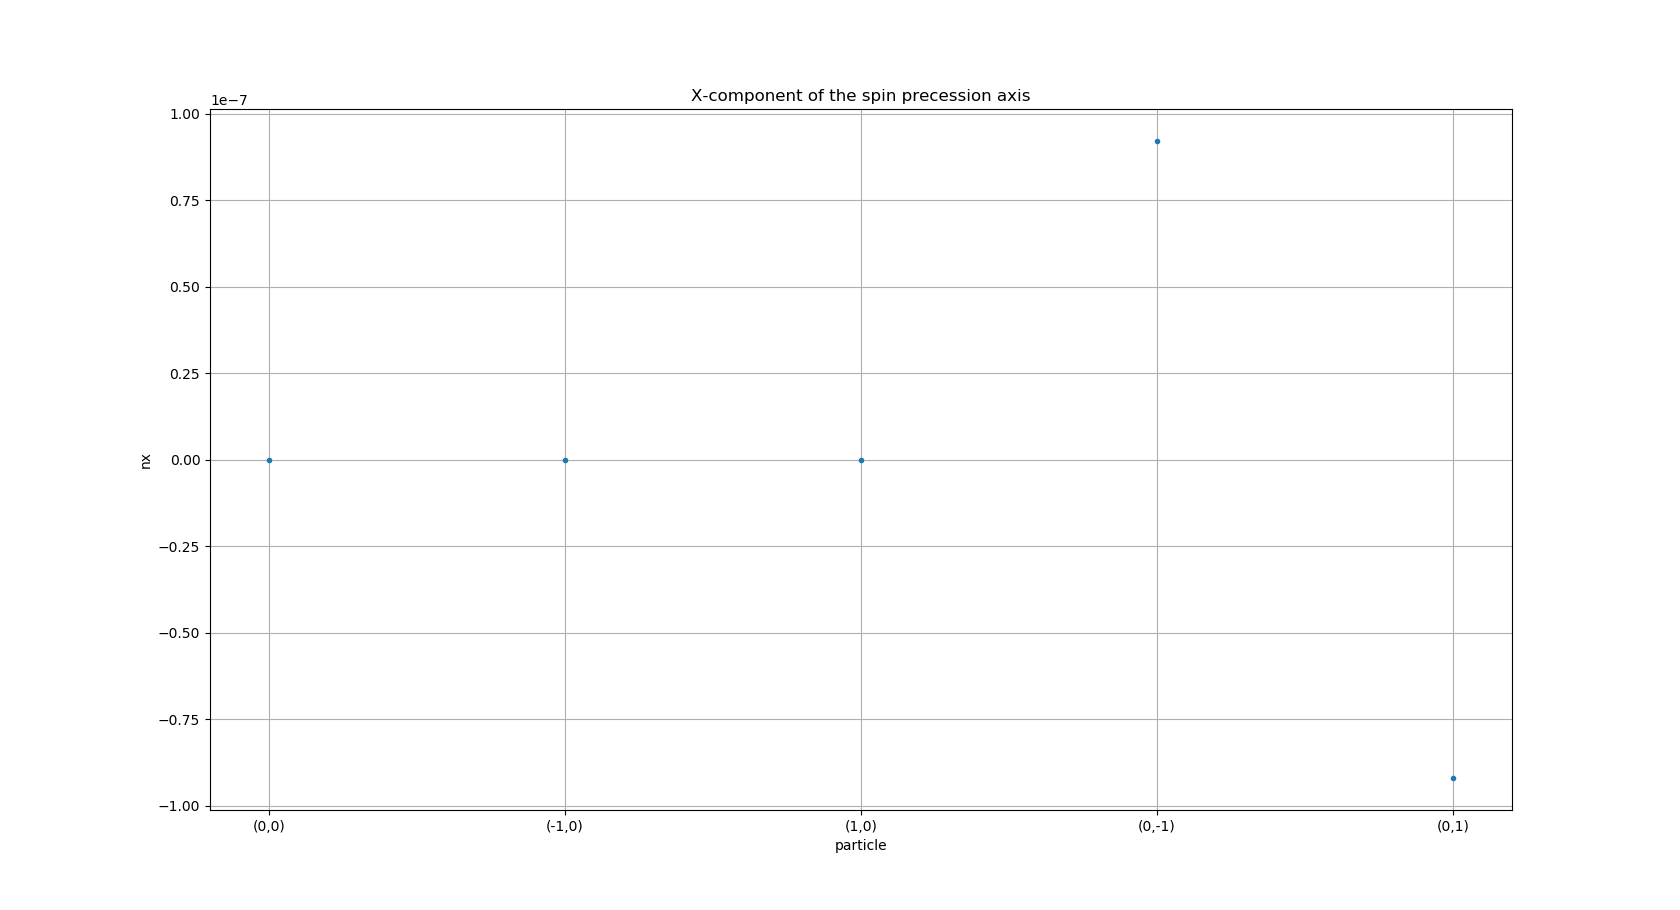
\includegraphics[width=\linewidth]{img/effective_gamma_question_nx}
  \caption{}
\end{figure}
\begin{figure}[!h]
  \centering
  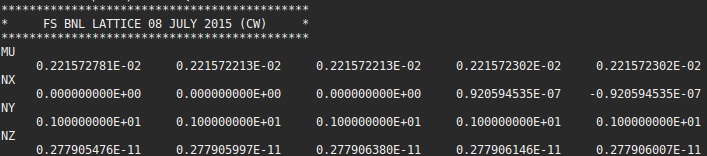
\includegraphics[width=\linewidth]{img/effective_gamma_question_screen}
  \caption{}
\end{figure}

\end{document}
